
\subsection{\HTSR Phenomenology: Predicting Model Quality via the \ALPHA metric}
\label{sxn:empirical-test_acc}

\begin{figure}[t]
  \center
  \subfigure[Batch size experiment]{
    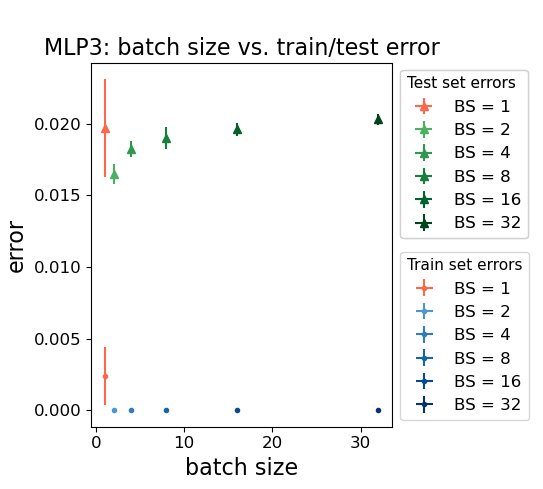
\includegraphics[width=6cm]{img/model_quality/mlp3_error_by_BS.png}
    \label{fig:mlp3-accuracies-bs}
  }
  \subfigure[Learning rate experiment]{
    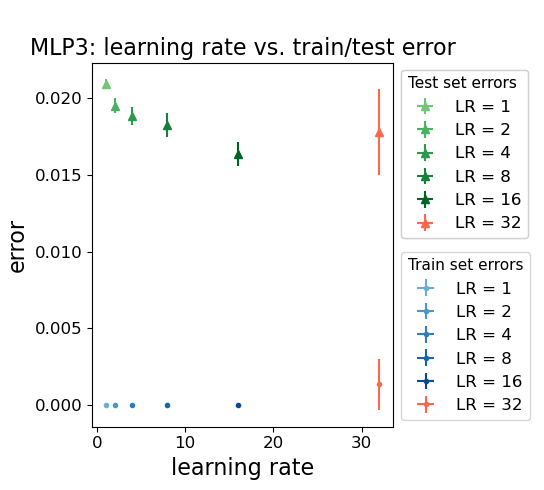
\includegraphics[width=6cm]{img/model_quality/mlp3_error_by_LR.png}
    \label{fig:mlp3-accuracies-lr}
  }
  \caption{Train / test errors in the MLP3 model as a function of batch size, and learning rate. Observe the inverse 
          relationship between batch size (a) and learning rate (b). As batch size decreases, test error generally 
          decreases, until batch size reached $bs=1$. Similarly, as learning rate increases, test error decreases until 
          $lr=32\times$ the SGD default value of $0.01$.
          \michael{More detailed and self-contained caption.}
          \michael{Also, lets be more clear about the LR, e.g., $32\times$ and so on.  Here and in the other figures consistently.}
          \chris{CH TODO: Redo this figure with $\times$ in the legend boxes.}
          \charles{@michael: redo it or close this out}
  }
  \label{fig:mlp3-accuracies}
\end{figure}

Here, we want to determine how the quality of our MLP3 model varies with the \ALPHA metric. 
From previous work~\cite{MM20a_trends_NatComm,MM21a_simpsons_TR,YTHx22_TR}, we expect that \ALPHA metrics for the FC1 and FC2 layers should be well-correlated with the test accuracy, while varying some suitable training knob, such as learning rate or batch size, that can modulate the test accuracy.% 
\footnote{Since we do not change the depth of the model here, we expect the \ALPHA metric to follow the \ALPHAHAT metric, also predicting the test accuracies~\cite{MM21a_simpsons_TR}.}

We vary the batch size from small to large, i.e., $bs\in[1,2,4,8,16,32]$, following the setup of previous work on the \HTSR~\Phenomenology~\cite{MM18_TR_JMLRversion}. 
We expect similar effects by varying the learning rate, as it is known that small batch sizes correspond directly to large learning rates~\cite{SKYL17_TR,WT11}. 
Thus, we conducted a second set of experiments where the learning rate was varied by a factor of 
$[1\times,2\times,4\times,8\times,16\times,32\times]$, relative to the SGD default value of $0.01$. 
% \michael{This is a little strange.  I added times, but we need to check and decide and do it consistently everywhere.  Is there a base rate, and we consider $1\times, 2\times \ldots 32\times$.  If we do that, then we need to add what is the baseline.  Lets be more clear, in the text and the caption.  }
% \chris{I added the default LR value.}
Adjusting the learning rate or batch size allows us to systematically vary the layer PL exponent $\alpha$ between roughly $2$ and $4$, i.e., within the range in which \SETOL should make the most reliable predictions. 
As an added benefit, it also allows us to use the very small batch size of $1$ to force the model into a state of over-regularization, which we also analyze below.
% \michael{Are we using the term over-regularization consistently everywhere?  We should define it very clearly somewhere above.}
% \chris{Over-regularizing is defined in Section~\ref{sxn:underfitting}, and it means $\alpha$ is too low, or 
%         $\LAMBDADETX < \LAMBDAPL$. Ive changed terms ``over-fit/\OverRegularized to just ``\OverRegularized.
% }

%%(In the HTSR \Phenomenology and the $5+1$ Phases-of-Training, and with how \WW~currently fits the ESDs, and barring additional spurious effects, this over-fitting regime corresponds to \VeryHeavyTailed (VHT) ESDs, with $\alpha<2$, which corresponds to a different HT \Universality class than $\alpha \in [2,4]$~\cite{MM18_TR_JMLRversion}.)

Consider Figure~\ref{fig:mlp3-accuracies}, which plots the final train and test accuracies as a function of the hyperparameter (batch size or learning rate) used during training for the MLP3 model.
Figure~\ref{fig:mlp3-accuracies-bs} varies batch size, and Figure~\ref{fig:mlp3-accuracies-lr} varies learning rate.
Recall that error bars represent one standard deviation taken over $5$ independent starting random seeds. 
In Figure~\ref{fig:mlp3-accuracies-bs}, we see that by decreasing the batch size ($bs$), and holding other knobs constant, we can systematically improve the train and test accuracy, up to a point. 
In particular, for $bs \ge 2$, both the test and train accuracies increase with decreasing batch size, consistent with previous work~\cite{MM18_TR_JMLRversion}.
Further decrease beyond $bs=2$ leads to \emph{lower} model quality, i.e., larger error and larger error variability.
In Figure~\ref{fig:mlp3-accuracies}, we see that increasing the learning rate ($lr$) by a factor $x$ has an exactly analogous effect as decreasing the batch size by $1/x$.% 
\footnote{One could, of course, mitigate this by fiddling with other knobs of the training process, but that is not our goal.  Our goal here is not to use a toy model to demonstrate the properties and predictions of \SETOL.}

\begin{figure}[t]
    \centering
    \subfigure[$\alpha_{FC1}$]{
        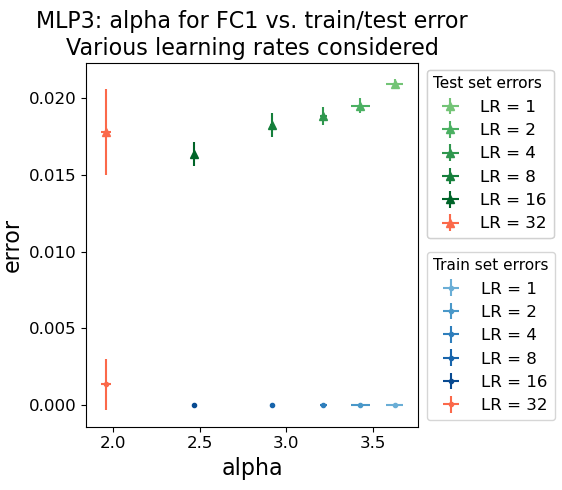
\includegraphics[width=6cm]{img/model_quality/mlp3_alpha_FC1_by_LR.png}
        \label{fig:mlp3-alpha-fc1-by-lr}
    } 
%    \subfigure[$\Delta \lambda_{min}$ FC1]{
%        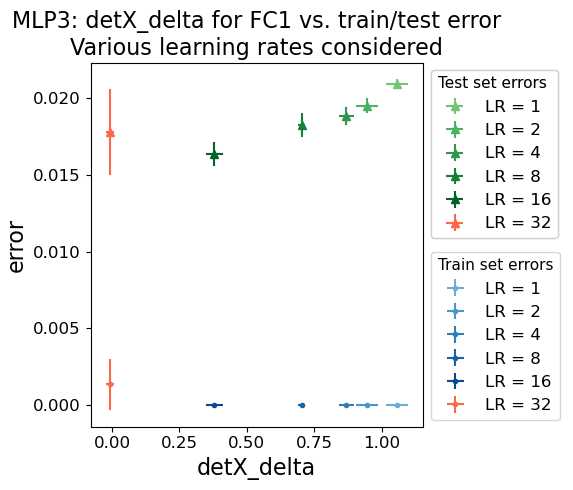
\includegraphics[width=6cm]{img/model_quality/mlp3_detX_Delta_FC1_by_LR.png}
%        \label{fig:mlp3-detx-delta-fc1-by-lr}
%    } \\
    \subfigure[$\alpha_{FC2}$]{
        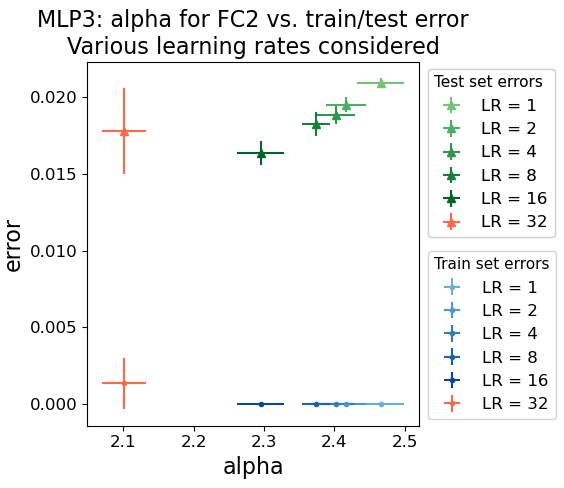
\includegraphics[width=6cm]{img/model_quality/mlp3_alpha_FC2_by_LR.png}
        \label{fig:mlp3-alpha-fc2-by-lr}
    } 
%    \subfigure[$\Delta \lambda_{min}$ FC1]{
%        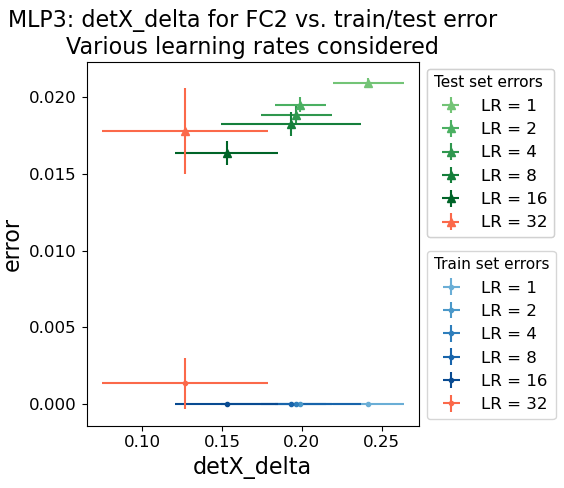
\includegraphics[width=6cm]{img/model_quality/mlp3_detX_Delta_FC2_by_LR.png}
%        \label{fig:mlp3-detx-delta-fc2-by-lr}
%    }  

    \caption{
            Train / test errors in the MLP3 model in the {\bf \emph{\LearningRate}} experiment as a function of $\alpha_{FC1}$ (a) and $\alpha_{FC2}$ (b). 
%            \michael{I like that ``\LearningRate is in bold, since it highlights what the caption is about.  Lets do that and similar things consistently everywhere to make captions easily understandable.}
            Observe the regular downward progression of $\alpha$ and error as the learning 
            rate increased in both (a) and (b). When learning rate was $32\times$, (shown in red), $\alpha_{FC1}$ fell 
            below $2$, coinciding with a drastic increase in both train and test error. The results here almost 
            perfectly replicate those of the Batch Size experiment, shown in Figure~\ref{fig:mlp3-alphas-bs}.
            \michaeladdressed{Maybe put X and Y on same axes for different figures; would you do that and see how it looks. Ditto 
              for Figure~\ref{fig:mlp3-alphas-bs}.}
            \charles{@michael: No}
    }
 \label{fig:mlp3-alphas-lr}
\end{figure}

The transition between $lr=16\times$ (or $bs=2$), which is locally optimal for the setting of other hyperparameters, and $lr=32\times$ normal (or $bs=1$), which is not, provides a demonstration of a distinct change in the behavior of \ALPHA, concordant with the sudden increase in the error and error variability. 
To explore this in the context of \SETOL, consider Figure~\ref{fig:mlp3-alphas-lr} and Figure~\ref{fig:mlp3-alphas-bs}, which plot error as a function of \ALPHA, for different learning rates and batch sizes, respectively.

Figure~\ref{fig:mlp3-alphas-lr} plots the \ALPHA metrics $\alpha_{FC1}$ and $\alpha_{FC2}$, as learning rate is varied, demonstrating that both metrics are well-correlated with the test accuracies, for all learning rates less than $16\times$ normal. 
In particular, as we drive \ALPHA in FC1 down to an \Ideal value of $\alpha\simeq 2$, the test error decreases monotonically (Figure~\ref{fig:mlp3-alpha-fc1-by-lr}).
Beyond that point, further decrease of the batch size sees \ALPHA decrease below its \Ideal value of $2$ in the FC1 layer.
This corresponds not only with \emph{higher errors}, but also with \emph{larger error bars}, on both train and test error. 
The dramatic increase in train error and train error variability is particularly telling, because it suggests that when 
$\alpha_{FC1}$ passes below $2$, the model enters into a ``glassy state, and is unable to relax down to $0$ train error.

In Figure~\ref{fig:mlp3-alpha-fc2-by-lr}, we consider \ALPHA for FC2, and we see that $\alpha_{FC2}$ approaches $2$, but 
does not reach it, even for $lr=32\times$. This failure to achieve $\alpha_{FC2} \approx 2$, along with the much greater size 
of FC1, (See Table~\ref{tab:mlp3},) suggests that FC1 is the critical layer for the models performance. 
This also highlights some of the interplay between the layers, (which is not captured by a single layer theory) -- as $\alpha_{FC1}$ has narrow error bars throughout, $\alpha_{FC2}$ shows much more variation by way of its wider error bars. 
Thus, while model accuracy kept improving as learning rate increased up to $16\times$, this was likely driven by a better $\alpha_{FC1}$, more than by $\alpha_{FC2}$. 

In Figure~\ref{fig:mlp3-alphas-bs}, we consider batch size, and we see a near identical replication of these results, in terms of the relation of train error, test error and \ALPHA in the two layers. 
Consequently, the remainder of the experiments will focus on the learning rate experiment, as both produced substantially the same results.

\begin{figure}[t] %[h]
    \centering
    \subfigure[$\alpha_{FC1}$]{
        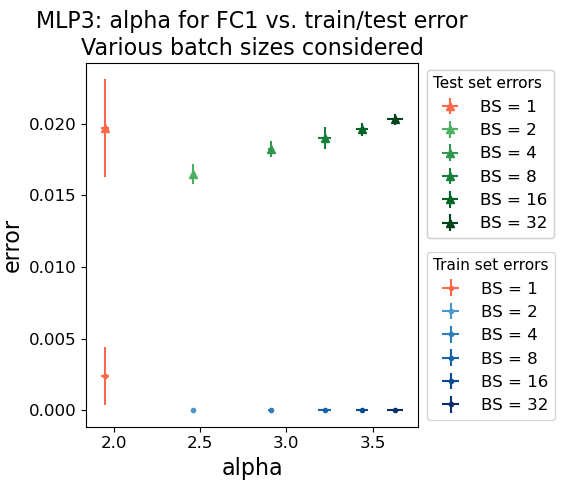
\includegraphics[width=6cm]{img/model_quality/mlp3_alpha_FC1_by_BS.png}
        \label{fig:mlp3-alpha-fc1-by-bs}
    } 
%    \subfigure[$\Delta \lambda_{min}$ FC1]{
%        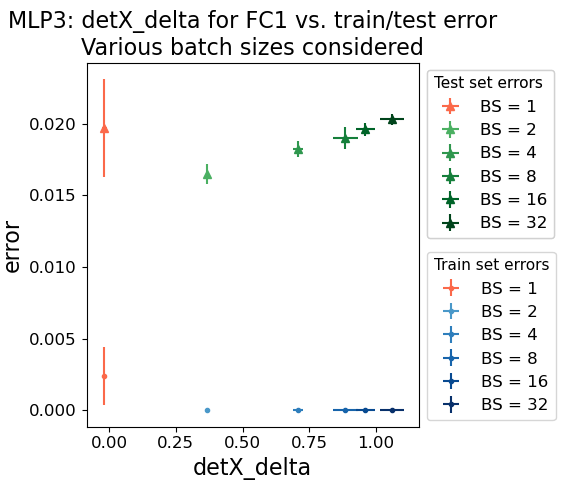
\includegraphics[width=6cm]{img/model_quality/mlp3_detX_Delta_FC1_by_BS.png}
%        \label{fig:mlp3-detx-delta-fc1-by-bs}
%    } \\
    \subfigure[$\alpha_{FC2}$]{
        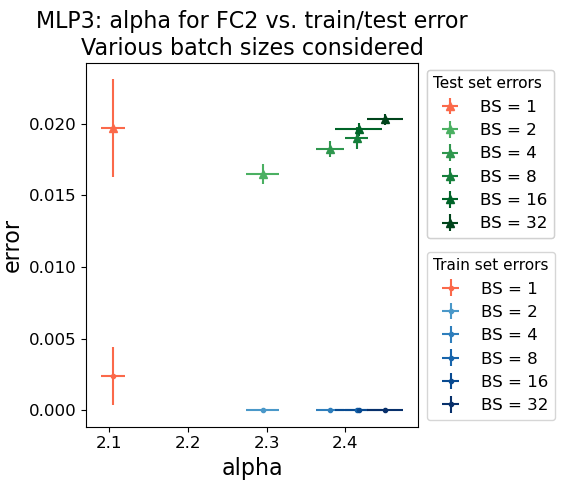
\includegraphics[width=6cm]{img/model_quality/mlp3_alpha_FC2_by_BS.png}
        \label{fig:mlp3-alpha-fc2-by-bs}
    } 
%    \subfigure[$\Delta \lambda_{min}$ FC1]{
%        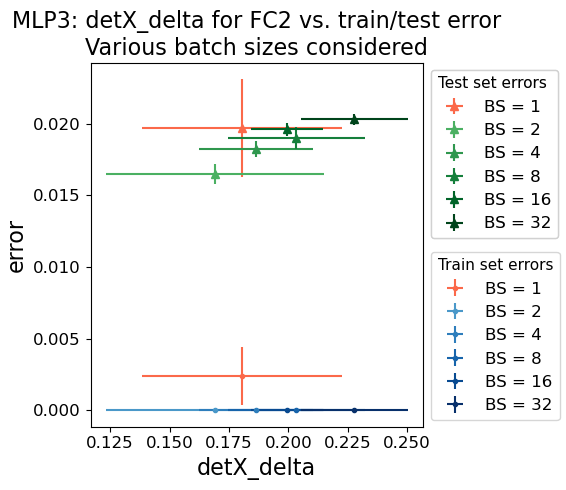
\includegraphics[width=6cm]{img/model_quality/mlp3_detX_Delta_FC2_by_BS.png}
%        \label{fig:mlp3-detx-delta-fc2-by-bs}
%    }  

    \caption{
            Train / test errors in the MLP3 model in the {\bf Batch Size} experiment as a function of $\alpha_{FC1}$ 
            (a) and $\alpha_{FC2}$ (b). Observe the regular downward progression of $\alpha$ and error as the batch size
            decreased in both (a) and (b). When batch size was $1$, (shown in red), $\alpha_{FC1}$ fell below $2$, 
            coinciding with a drastic increase in both train and test error. The results here almost perfectly 
            replicate those of the \LearningRate experiment, shown in Figure~\ref{fig:mlp3-alphas-lr}.
    }
 \label{fig:mlp3-alphas-bs}
\end{figure}



